% !TEX root =  master.tex

\section{Multilevel Queue Scheduling}
Aufbauen auf anderen Prozess-Schedulern, wie bspw. dem zuvor beschriebenen First Come First Serve oder Round-Robin Prinzip gibt es weitere Verfahren, welche durch eine erweiterte Komplexität beabsichtigen, zuvor dargelegte Prinzipien und Stärken zu vereinen und Schwächen zu überwinden. Eines dieser Verfahren ist das Multilevel Queue Scheduling. Es handelt sich hierbei um einen Algorithmus, bei welchem Prozesse abhängig ihrer Eigenschaften in verschiedene Kategorien eingeteilt und anschließend entsprechend mit unterschiedlicher Priorität bearbeitet werden. Es soll somit durch das Priorisieren von zeitkritischen Aufgaben und der dynamischen Ressourcenzuweisung dem Ziel einer gerechten und effizienten Prozessverwaltung weiter nähergekommen werden.
Beim Multilevel Queue Scheduling Verfahren werden zunächst die aktuell offenen, zu bearbeitenden Prozesse unterschiedlichen Warteschlangen dauerhaft zugewiesen. Diese Einteilung kann auf Grundlage unterschiedlicher Kriterien geschehen und ausschlaggebend können beispielsweise Speichergröße, Prozesspriorität oder der Prozesstyp sein. Eine einfache Aufteilung ist die Zuordnung in Vordergrundaktivitäten und Hintergrundaktivitäten, sodass die eine Gruppe interaktive Prozesse umfasst, welche zeitnah abgearbeitet werden müssen und die andere Gruppe eher statische Prozesse, die ggf. auch länger für die Bearbeitung benötigen. Jede der so geformten Warteschlagen kann unabhängig, auf unterschiedliche Art und Weise bearbeitet werden und verfügt über einen eigenen Scheduling-Algorithmus. So ist es üblich, die Warteschlange für Vordergrundaktivitäten nach dem Round Robin Prinzip abgearbeitet wird, während bei der anderen Warteschlange mit Hintergrundaktivitäten das First Come First Serve Prinzip Anwendung findet. %Ggf. hier noch eine Begründung geben
Neben den unterschiedlichen Verfahren, die innerhalb der Wartschlangen stattfinden, gibt es ein einfaches Scheduling-Verfahren zur Verwaltung der Warteschlangen untereinander. Dieses ist für gewöhnlich mit einer festen Priorisierung und präemptiv implementiert. Das bedeutet, dass Warteschlangen absolute Prioritäten über anderen haben und eine höher priorisierte Wartschlange zunächst vollständig abgearbeitet wird, gleichzeitig die Bearbeitung einer niedrig priorisierten Warteschlange aber zugunsten neuer Prozesse in einer anderen Schlange unterbrochen werden kann \cite[S.214 f.]{Silberschatz.2019}.

\begin{algorithm}
	\caption{Multilevel-Queue-Scheduling} \label{algo:mlq}
	\begin{algorithmic}[1]

		\State \textbf{Initialize:} $n$ Warteschlangen $Q_1, Q_2, \ldots, Q_n$, jede mit ihrem eigenen Scheduling-Algorithmus $S_1, S_2, \ldots, S_n$
		\State Zuweisung von jedem Prozess, basierend auf seinem Typ oder seiner Priorität, in eine Warteschlange

		\While{es noch zu abzuarbeitende Prozesse gibt}
		\For{jede Warteschlange $Q_i$ in Prioritätsreihenfolge}
		\If{$Q_i$ nicht leer ist}
		\State Wähle einen Prozess $P$ aus $Q_i$ mithilfe des Scheduling-Algorithmus $S_i$
		\State Führe Prozess $P$ aus
		\If{Prozess $P$ abgeschlossen ist}
		\State Entferne $P$ aus $Q_i$
		\ElsIf{ein Prozess mit höherer Priorität eintrifft}
		\State Unterbreche $P$ und füge ihn zurück in $Q_i$ ein
		\EndIf
		\EndIf
		\EndFor
		\EndWhile

	\end{algorithmic}
\end{algorithm}

Der Algorithmus in \ref{algo:mlq} stellt dar, wie das \ac{MLQ}-Verfahren im Allgemeinen mit einer beliebigen Anzahl an Warteschlangen abläuft.
In einem vereinfachen Beispiel mit zwei Warteschlangen würden zunächst die Vordergrundaktivitäten nach dem Round Robin Verfahren abgearbeitet und sobald diese Wartschlange leer ist, die Hintergrundaktivitäten mittels First Come First Serve erledigt werden. Tritt während der Bearbeitung der Hintergrundaktivitäten ein Vordergrundprozess auf, wird diese Bearbeitung solange unterbrochen, bis wieder alle Vordergrundaktivitäten abgearbeitet sind.
Das Verfahren ist hierbei nicht wie in diesem Beispiel auf zwei Warteschlangen beschränkt, sondern kann um eine Vielzahl an Schlangen für verschiedene Prozesseigenschaften erweitert werden, wie in Abbildung \ref{fig:mlq_queues} dargestellt.
\begin{figure}[ht]
	\centering
	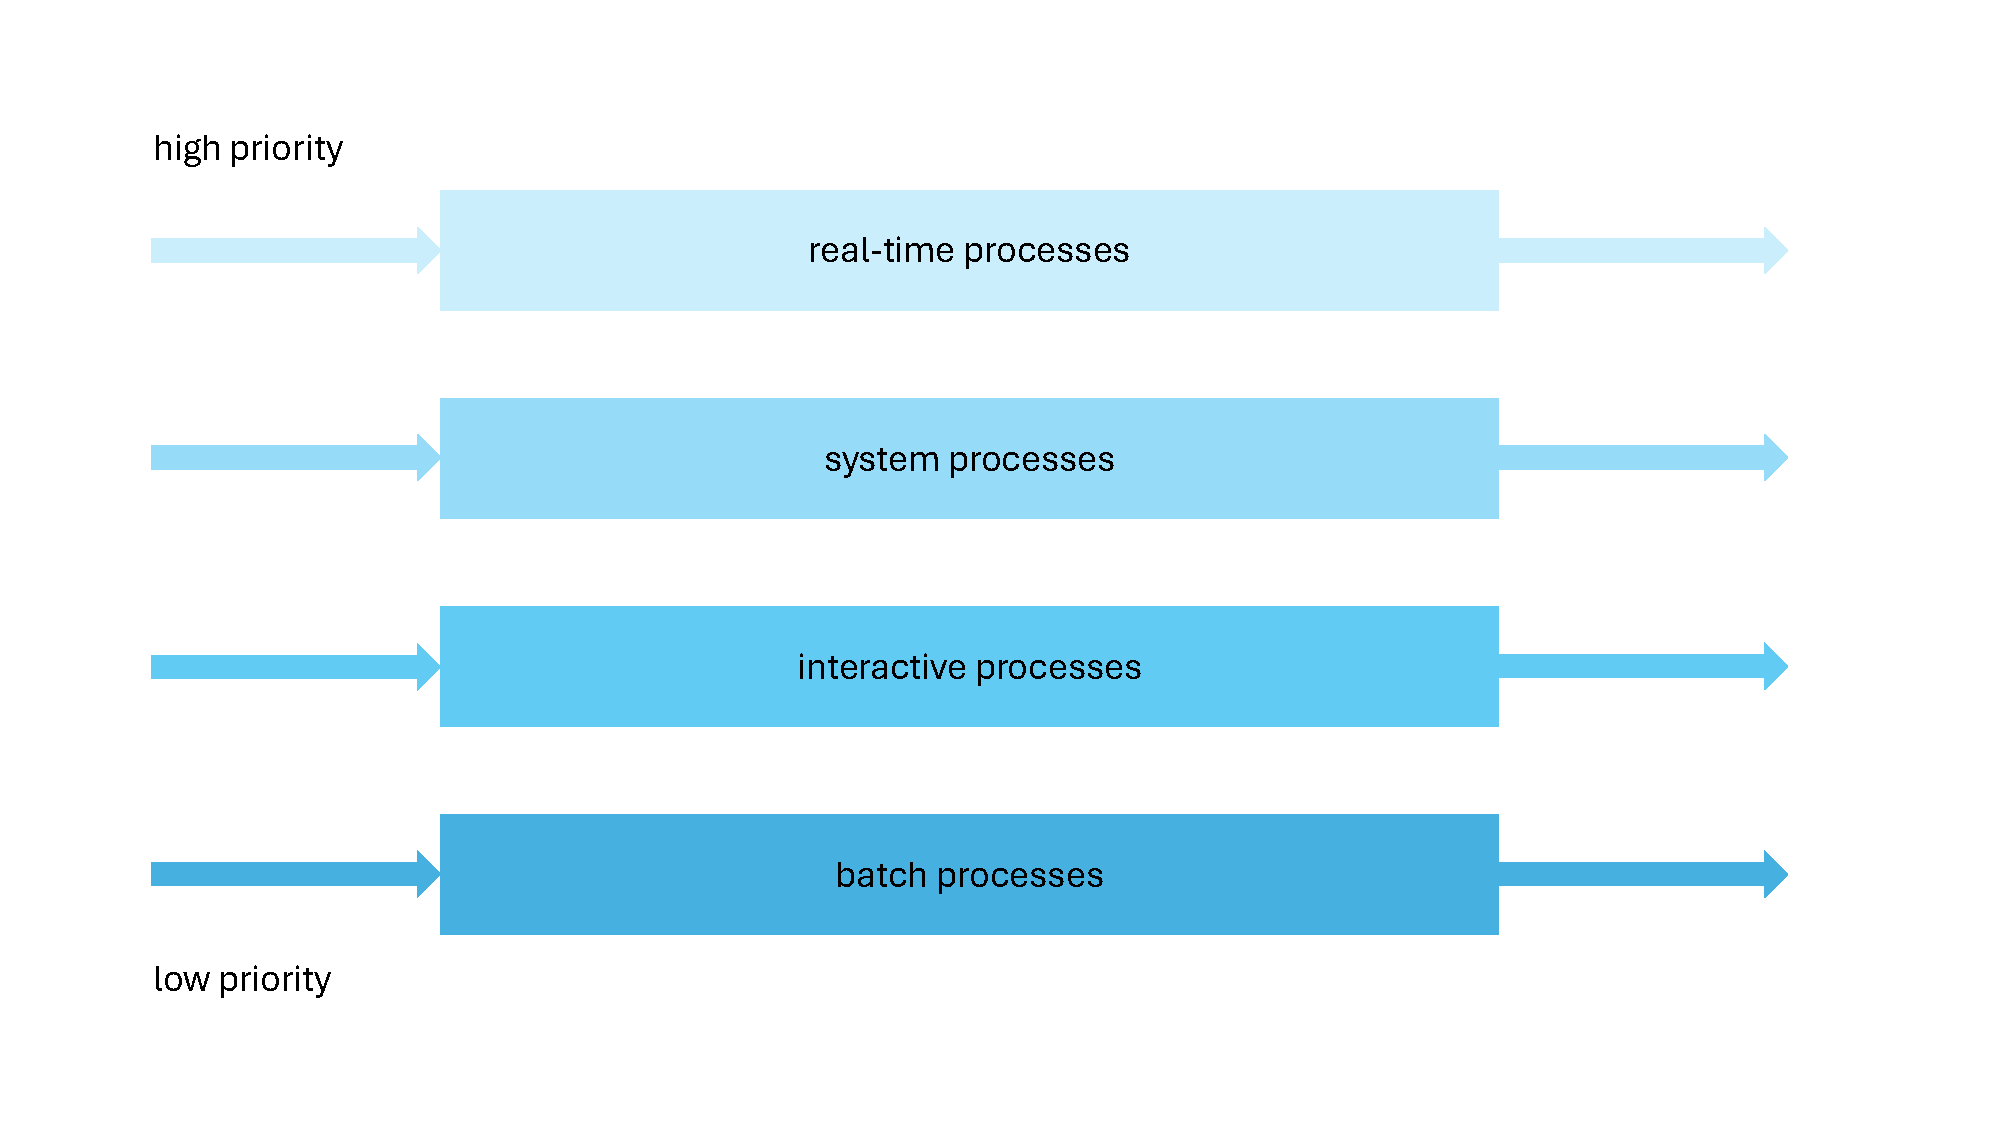
\includegraphics[width=\linewidth]{img/mlq.pdf}
	\caption{Darstellung des \ac{MLQ}-Schedulings mit mehreren Warteschlangen \cite[S.215]{Silberschatz.2019}}
	\label{fig:mlq_queues}
\end{figure}

Das Multilevel Queue Scheduling Verfahren bietet aufgrund seiner erweiterten Komplexität gegenüber herkömmlichen deutlich einfacheren Verfahren einige Vorteile, aber auch Nachteile. So ist positiv zu bemerken, dass die Reaktionszeit des Systems durch die effizientere Ressourcenallokation reduziert werden kann und die Nutzererfahrung durch die schnellere Abarbeitung von interaktiven Prozessen verbessert wird. Des Weiterem kann mit diesem Verfahren unter den richtigen Umständen der Durchsatz gesteigert werden und das System ggf. auch Prozesse unterschiedlicher Schlangen gleichzeitig ausführen, welches zu der Effizienz des Systems beiträgt. Negativ zu betrachten sind hingegen die erhöhte Komplexität beim Design eines effizienten Systems sowie der zusätzliche Arbeitsaufwand zur Verwaltung der mehreren Warteschlangen untereinander, welcher die Performance des Systems wiederum lindern kann. Ein weiteres Problem ist das „Verhungern“ von Prozessen in einer Warteschlange mit niedrigerer Priorität, welches auftreten kann, wenn zu viele, große Prozesse in anderen Schlangen zuerst abgearbeitet werden müssen.
Um diesem Nachteilen des „Verhungerns“ von Prozessen entgegenzuwirken, gibt es Weiterentwicklungen der einfachen Multilevel Queue wie beispielsweise das heute verbreitete Multilevel Feedback Queue Verfahren. Hier sind die Prozesse nicht komplett fest einer Warteschlange zugeordnet, sondern können auch zu einem späteren Zeitpunkt noch in eine andere Schlange verschoben werden. Dies hilft dabei, dass das System besser auf die Bearbeitungszeiten der Prozesse reagieren kann und keine Prozesse vernachlässigt werden.
%könnte man ggf. noch im Detail ausführen, falls wir mehr Text brauchen


%%%%
%Der zentrale Vorteil von \ac{MLQ} liegt in dessen Flexibilität und Effizienz bei der Behandlung verschiedener Prozesstypen. Beispielsweise können Systemprozesse, interaktive Prozesse und Batch-Prozesse in verschiedenen Warteschlangen mit entsprechenden Prioritäten und Scheduling-Strategien verwaltet werden. Hierdurch wird eine bessere Anpassung an die Anforderungen spezifischer Prozesstypen erreicht, was zu einer verbesserten Gesamtleistung des Systems führt. % Tanenbaum und Bos (2014) 

%Ein Nachteil von \ac{MLQ} liegt allerdings in seiner Komplexität, sowohl in der Implementierung als auch im Management. Die korrekte Einordnung von Prozessen in Warteschlangen und die Auswahl geeigneter Scheduling-Algorithmen für jede Warteschlange erfordern sorgfältige Planung und ständige Anpassung. Eine nachteilige Auswahl und Konfiguration dieser Algorithmen kann zu einem erhöhten Overhead führen und die Systemeffizienz negativ beeinträchtigen. % Stallings (2012)

%Trotz dieser Herausforderungen ist \ac{MLQ} ein beliebter Scheduling Algorithmus in Betriebssystemen, insbesondere dort, wo eine Vielzahl unterschiedlicher Prozesse und Anforderungen effizient verwaltet werden muss.

%\textit{Referenzen:}
%\begin{itemize}
%	\item Silberschatz, A., Galvin, P. B., \& Gagne, G. (2018). Operating System Concepts. Wiley.
%	\item Tanenbaum, A. S., \& Bos, H. (2014). Modern Operating Systems. Pearson.
%	\item Stallings, W. (2012). Operating Systems: Internals and Design Principles. Prentice Hall.
%\end{itemize}


